\documentclass[10pt,a4paper]{article}

\usepackage[spanish,activeacute,es-tabla]{babel}
\usepackage[utf8]{inputenc}
\usepackage{ifthen}
\usepackage{listings}
\usepackage{dsfont}
\usepackage{subcaption}
\usepackage{amsmath}
\usepackage[strict]{changepage}
\usepackage[top=1cm,bottom=2cm,left=1cm,right=1cm]{geometry}%
\usepackage{color}%
\newcommand{\tocarEspacios}{%
	\addtolength{\leftskip}{3em}%
	\setlength{\parindent}{0em}%
}

% Especificacion de procs

\newcommand{\In}{\textsf{in }}
\newcommand{\Out}{\textsf{out }}
\newcommand{\Inout}{\textsf{inout }}

\newcommand{\encabezadoDeProc}[4]{%
	% Ponemos la palabrita problema en tt
	%  \noindent%
	{\normalfont\bfseries\ttfamily proc}%
	% Ponemos el nombre del problema
	\ %
	{\normalfont\ttfamily #2}%
	\
	% Ponemos los parametros
	(#3)%
	\ifthenelse{\equal{#4}{}}{}{%
		% Por ultimo, va el tipo del resultado
		\ : #4}
}

\newenvironment{proc}[4][res]{%
	
	% El parametro 1 (opcional) es el nombre del resultado
	% El parametro 2 es el nombre del problema
	% El parametro 3 son los parametros
	% El parametro 4 es el tipo del resultado
	% Preambulo del ambiente problema
	% Tenemos que definir los comandos requiere, asegura, modifica y aux
	\newcommand{\requiere}[2][]{%
		{\normalfont\bfseries\ttfamily requiere}%
		\ifthenelse{\equal{##1}{}}{}{\ {\normalfont\ttfamily ##1} :}\ %
		\{\ensuremath{##2}\}%
		{\normalfont\bfseries\,\par}%
	}
	\newcommand{\asegura}[2][]{%
		{\normalfont\bfseries\ttfamily asegura}%
		\ifthenelse{\equal{##1}{}}{}{\ {\normalfont\ttfamily ##1} :}\
		\{\ensuremath{##2}\}%
		{\normalfont\bfseries\,\par}%
	}
	\renewcommand{\aux}[4]{%
		{\normalfont\bfseries\ttfamily aux\ }%
		{\normalfont\ttfamily ##1}%
		\ifthenelse{\equal{##2}{}}{}{\ (##2)}\ : ##3\, = \ensuremath{##4}%
		{\normalfont\bfseries\,;\par}%
	}
	\renewcommand{\pred}[3]{%
		{\normalfont\bfseries\ttfamily pred }%
		{\normalfont\ttfamily ##1}%
		\ifthenelse{\equal{##2}{}}{}{\ (##2) }%
		\{%
		\begin{adjustwidth}{+5em}{}
			\ensuremath{##3}
		\end{adjustwidth}
		\}%
		{\normalfont\bfseries\,\par}%
	}
	
	\newcommand{\res}{#1}
	\vspace{1ex}
	\noindent
	\encabezadoDeProc{#1}{#2}{#3}{#4}
	% Abrimos la llave
	\par%
	\tocarEspacios
}
{
	% Cerramos la llave
	\vspace{1ex}
}

\newcommand{\aux}[4]{%
	{\normalfont\bfseries\ttfamily\noindent aux\ }%
	{\normalfont\ttfamily #1}%
	\ifthenelse{\equal{#2}{}}{}{\ (#2)}\ : #3\, = \ensuremath{#4}%
	{\normalfont\bfseries\,;\par}%
}

\newcommand{\pred}[3]{%
	{\normalfont\bfseries\ttfamily\noindent pred }%
	{\normalfont\ttfamily #1}%
	\ifthenelse{\equal{#2}{}}{}{\ (#2) }%
	\{%
	\begin{adjustwidth}{+2em}{}
		\ensuremath{#3}
	\end{adjustwidth}
	\}%
	{\normalfont\bfseries\,\par}%
}

% Tipos

\newcommand{\nat}{\ensuremath{\mathds{N}}}
\newcommand{\ent}{\ensuremath{\mathds{Z}}}
\newcommand{\float}{\ensuremath{\mathds{R}}}
\newcommand{\bool}{\ensuremath{\mathsf{Bool}}}
\newcommand{\cha}{\ensuremath{\mathsf{Char}}}
\newcommand{\str}{\ensuremath{\mathsf{String}}}

% Logica

\newcommand{\True}{\ensuremath{\mathrm{true}}}
\newcommand{\False}{\ensuremath{\mathrm{false}}}
\newcommand{\Then}{\ensuremath{\rightarrow}}
\newcommand{\Iff}{\ensuremath{\leftrightarrow}}
\newcommand{\implica}{\ensuremath{\longrightarrow}}
\newcommand{\IfThenElse}[3]{\ensuremath{\mathsf{if}\ #1\ \mathsf{then}\ #2\ \mathsf{else}\ #3\ \mathsf{fi}}}
\newcommand{\yLuego}{\land _L}
\newcommand{\y}{\land}
\newcommand{\oLuego}{\lor _L}
\newcommand{\implicaLuego}{\implica _L}

\newcommand{\cuantificador}[5]{%
	\ensuremath{(#2 #3: #4)\ (%
		\ifthenelse{\equal{#1}{unalinea}}{
			#5
		}{
			$ % exiting math mode
			\begin{adjustwidth}{+2em}{}
				$#5$%
			\end{adjustwidth}%
			$ % entering math mode
		}
		)}
}

\newcommand{\existe}[4][]{%
	\cuantificador{#1}{\exists}{#2}{#3}{#4}
}
\newcommand{\paraTodo}[4][]{%
	\cuantificador{#1}{\forall}{#2}{#3}{#4}
}

%listas

\newcommand{\TLista}[1]{\ensuremath{seq \langle #1\rangle}}
\newcommand{\lvacia}{\ensuremath{[\ ]}}
\newcommand{\lv}{\ensuremath{[\ ]}}
\newcommand{\longitud}[1]{\ensuremath{|#1|}}
\newcommand{\cons}[1]{\ensuremath{\mathsf{addFirst}}(#1)}
\newcommand{\indice}[1]{\ensuremath{\mathsf{indice}}(#1)}
\newcommand{\conc}[1]{\ensuremath{\mathsf{concat}}(#1)}
\newcommand{\cab}[1]{\ensuremath{\mathsf{head}}(#1)}
\newcommand{\cola}[1]{\ensuremath{\mathsf{tail}}(#1)}
\newcommand{\sub}[1]{\ensuremath{\mathsf{subseq}}(#1)}
\newcommand{\en}[1]{\ensuremath{\mathsf{en}}(#1)}
\newcommand{\cuenta}[2]{\mathsf{cuenta}\ensuremath{(#1, #2)}}
\newcommand{\suma}[1]{\mathsf{suma}(#1)}
\newcommand{\twodots}{\ensuremath{\mathrm{..}}}
\newcommand{\masmas}{\ensuremath{++}}
\newcommand{\matriz}[1]{\TLista{\TLista{#1}}}
\newcommand{\seqchar}{\TLista{\cha}}
\newcommand{\seqr}{\TLista{\float}}
\newcommand{\seqn}{\TLista{\nat}}
\newcommand{\seqB}{\TLista{\bool}}


\renewcommand{\lstlistingname}{Código}
\lstset{% general command to set parameter(s)
	language=Java,
	morekeywords={endif, endwhile, skip},
	basewidth={0.47em,0.40em},
	columns=fixed, fontadjust, resetmargins, xrightmargin=5pt, xleftmargin=15pt,
	flexiblecolumns=false, tabsize=4, breaklines, breakatwhitespace=false, extendedchars=true,
	numbers=left, numberstyle=\tiny, stepnumber=1, numbersep=9pt,
	frame=l, framesep=3pt,
	captionpos=b,
}

\usepackage{caratula} % Version modificada para usar las macros de algo1 de ~> https://github.com/bcardiff/dc-tex


\titulo{Trabajo pr\'actico 1: Especificaci\'on y WP}
\subtitulo{Fondo Monetario Com\'un}

\fecha{\today}

\materia{Algoritmos y Estructuras de Datos II}
\grupo{Grupo Debuggers}

\integrante{Apellido, Nombre1}{001/01}{email1@dominio.com}
\integrante{Apellido, Nombre2}{002/01}{email2@dominio.com}
\integrante{Apellido, Nombre3}{003/01}{email3@dominio.com}
\integrante{Azcurra, Mariano}{1321/21}{mariano.azcurra@hotmail.es}
% Pongan cuantos integrantes quieran

% Declaramos donde van a estar las figuras
% No es obligatorio, pero suele ser comodo
\graphicspath{{../static/}}

\begin{document}

\maketitle
\section{Aclaraciones generales}

\begin{itemize}
	\item Los ındices de las listas \textit{recursos, cooperan, trayectorias, apuestas, pagos, eventos} representa el identificador de los individuos.
	\item recursos: {\TLista{\float}} es la lista con el recurso de cada individuo.
 	\item cooperan:  {\TLista{\bool}} es la lista que indica True si el individuo en dicha posici\'on coopera.
        \item trayectorias: \TLista{\float} indica para cada individuo, en cada paso de tiempos, cu\'antos recursos (\float) cuenta.
        \item eventos:
        \item apuestas: 
        \item pagos: 
        \item Las personas que no cooperan no aportan nada al fondo monetario com\'un.
        \item Los recursos iniciales son positivos.
        \item Todos los pagos son positivos.
        \item Las apuestas de los individuos representan la proporci\'on de los recursos que los individuos invierten a cada una de los eventos posibles. Se puede tener apuestas
distintas para cada evento por cada individuo.
        \item Cada individuo apuesta siempre el mismo porcentaje por cada evento posible.

\end{itemize}
\section{Especificaci\'on}
\subsection{redistribucionDeLosFrutos}

%Lo principal: las fórmulas. Se puede poner en una linea, como $x_i = %x_{i-1} + x_{i-2}$, o ponerse más grande:

%\begin{equation}
%	\sum\limits_{i=0}^{n} i
%	\label{eq:1}
%\end{equation}

%Y se pueden citar ecuaciones con \verb|\eqref{nombreDeEq}|: %\eqref{eq:1}

%Ejemplo de itemizado:

%\begin{itemize}
%	\item Item 1
%	\item Item 2
%	\item Item 3
%\end{itemize}

%Ejemplo de enumerado con menor distancia entre items:

%\begin{enumerate} \setlength\itemsep{0cm}
%	\item Item 1
%	\item Item 2
%	\item Item 3
%\end{enumerate}

%Podemos escribir mucho texto. Mucho texto. Mucho texto. Mucho texto. %Mucho texto. Mucho texto. Mucho texto. Mucho texto. Mucho texto. %Mucho texto. Mucho texto.

%Otro párrafo. Otro párrafo. Otro párrafo. Otro párrafo. Otro párrafo. Otro párrafo. Otro párrafo. Otro párrafo. Otro párrafo. Otro párrafo. Otro párrafo. Otro párrafo. Otro párrafo.

%\vspace{0.3cm}

%Le agregamos una separación entre párrafos. Le agregamos una separación entre párrafos. Le agregamos una separación entre párrafos. Le agregamos una separación entre párrafos. Le agregamos una separación entre párrafos.

%\vspace{0.3cm}

%La tabla \ref{tab:ejemplo} es un ejemplo de cómo se hace una tabla.

%\begin{table}[h!]
%	\centering
%	\begin{tabular}{||l c c r||} 
%		\hline
%		Col1 & Col2 & Col2 & Col3 \\ [0.5ex] 
%		\hline\hline
%		1 & 6 & 87837 & 787 \\ 
%		2 & 7 & 78 & 5415 \\
%		3 & 545 & 778 & 7507 \\
%		5 & 88 & 788 & 6344 \\
%		\hline
%	\end{tabular}
%	\caption{Ejemplo de tabla}
%	\label{tab:ejemplo}
%\end{table}


%La figura \ref{fig:subfigs} es un ejemplo de cómo se agrega una imagen.

%\begin{figure}[ht]
%	\centering
%	
\includegraphics[width=0.6\textwidth]{logo_dc.jpg}
%	\caption{Ejemplo de figura}
%	\label{fig:ejemplo}
%\end{figure}

%\begin{figure}[ht!]
%	\begin{subfigure}{0.5\textwidth}
%		
\includegraphics[width=0.9\linewidth]{LaTeX-project} 
%		\caption{Logo de LaTeX}
%		\label{fig:subfig1}
%	\end{subfigure}
%	\begin{subfigure}{0.5\textwidth}
%		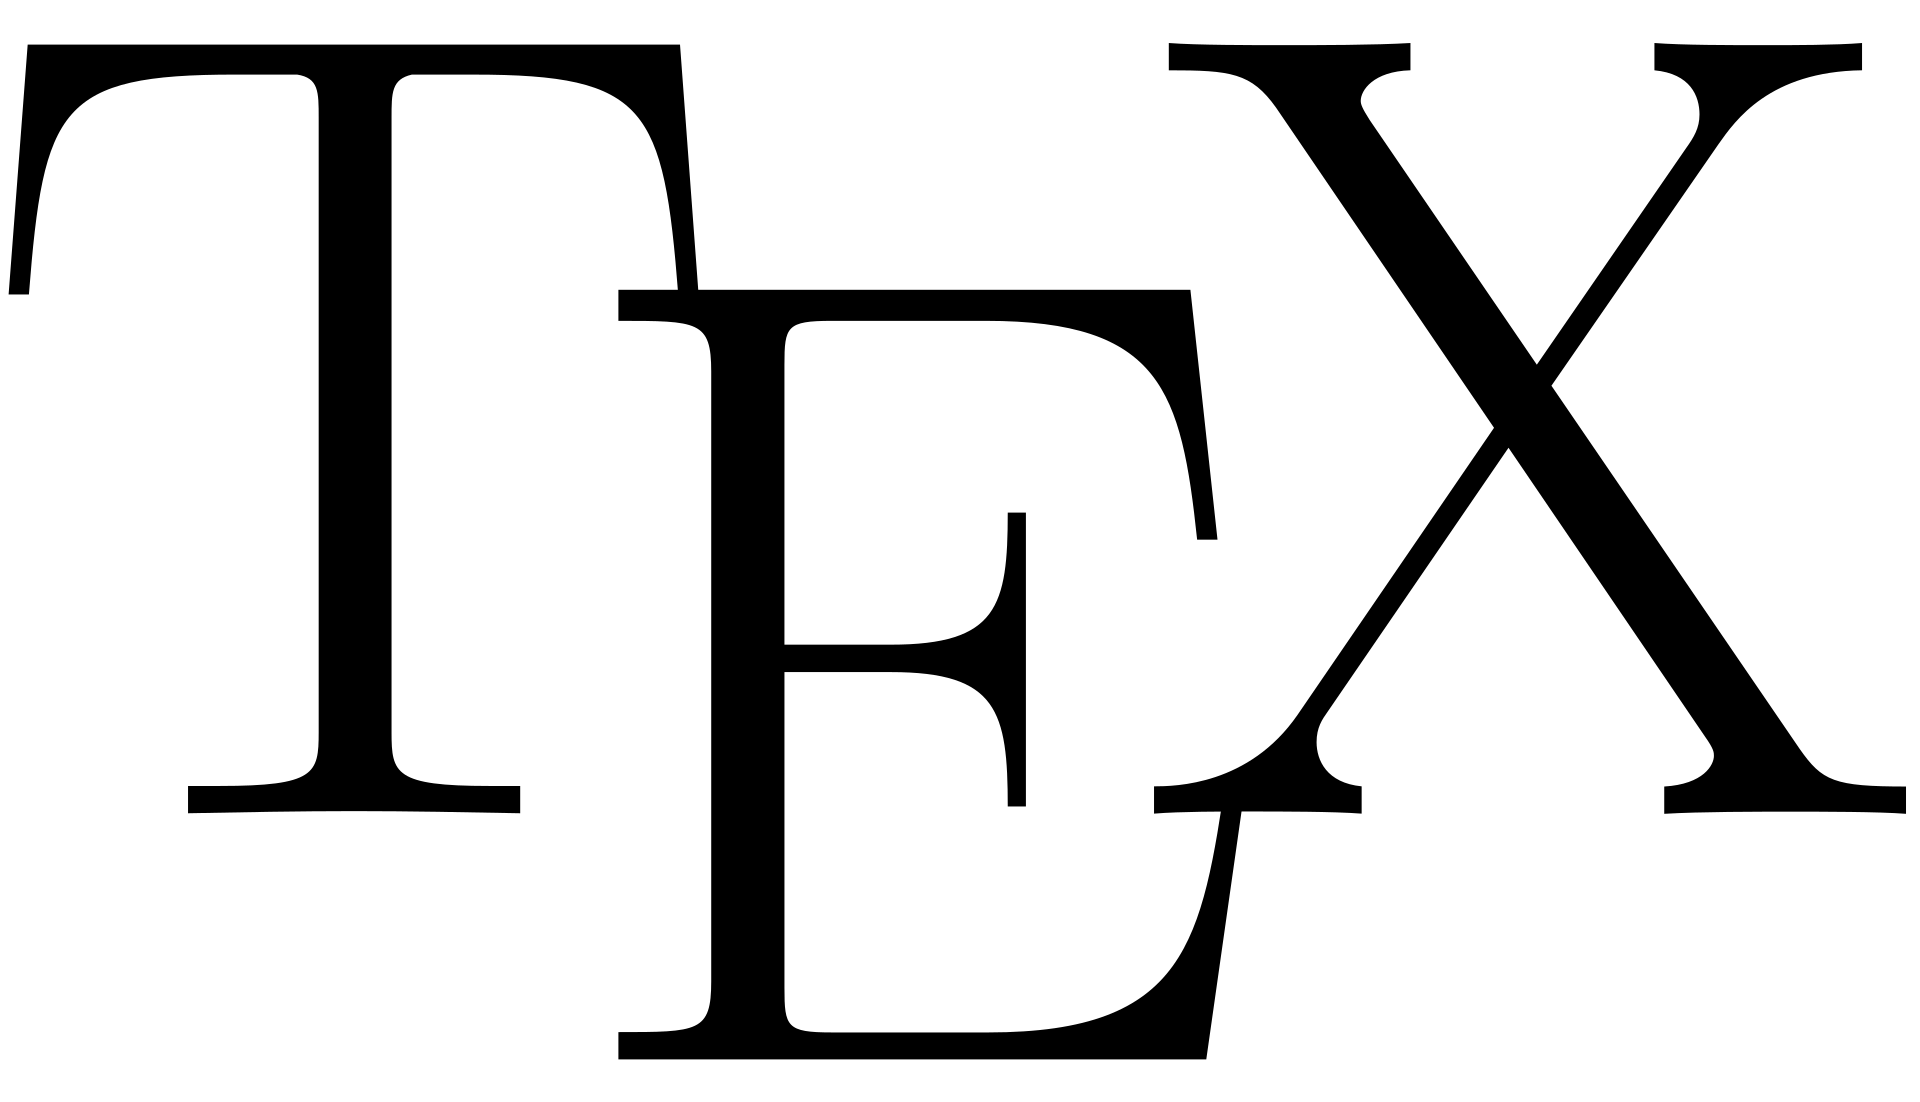
\includegraphics[width=0.7\linewidth]{TeX}
%		\caption{Logo de TeX}
%		\label{fig:subfig2}
%	\end{subfigure}
%	\caption{Ejemplo para poner dos figuras juntas. Y citarlas por separado a (\subref{fig:subfig1}) y (\subref{fig:subfig2}).}
	% OJO: el caption siempre va antes del label
	\label{fig:subfigs}
%\end{figure}



% Para hacer que quede todo en una misma linea, se puede usar minipage
%\begin{minipage}[t]{\textwidth}
%	\begin{lstlisting}[caption={Ejemplo de código (usando los estilos de la cátedra, ver las macros para más detalles)},label=code:for]
%res := 0;
%i := 0;
%while (i < s.size()) do
%	res := res + s[i];
%	i := i + 1
%endwhile
%	\end{lstlisting}
%\end{minipage}

%Si se pone un label al \verb|lstlisting|, se puede referenciar: Código \ref{code:for}.
\subsection{proc 2}
\subsection{proc 3}
\subsection{proc 4}
\subsection{individuoActualizaApuesta}

\begin{proc}{individuoActualizaApuesta}{
\In individuo: \nat,
\In recursos: \TLista{\float}, 
\In cooperan: \TLista{\bool}, 
\Inout apuestas: \Tlista{\TLista{\float}}, 
\In pagos: \Tlista{\TLista{\float}},
\In eventos: \Tlista{\nat}}
{\Tlista{\TLista{\float}}}
	%    \modifica{parametro1, parametro2,..}
	\requiere{apuestas = A_{0}}
	\asegura{|apuestas| = |A_{0}| \wedge \\ esApuestaValida(apuestas[individuo]) \wedge \\ 
 \begin{minipage}[t]{\textwidth}
 \paraTodo{j}{\ent}{0 \leq j < |apuestas[individuo]| \wedge j \neq i \implicaLuego  apuestas [j] =  A_{0}[j]} 
 \end{minipage} 
 \\ \wedge 
 \neg\existe{apuestaTeorica}{\TLista{\float}}{esApuestaValida(apuestaTeorica) \\
 \wedge 
 ganancias (individuo, apuestaTeorica, eventos, pagos[individuo],cooperan, recursos[individuo]) > \\  ganancias (individuo, apuestas[individuo], eventos, pagos[individuo],cooperan, recursos[individuo])}
}

\vspace{5mm}

	\aux{ganancias}{individuo: \nat, apuesta: \Tlista{\float}, eventos: \Tlista{\nat}, pagos: \Tlista{\float}, cooperan: \Tlista{Bool}, recursos: \Tlista{\float}}{\float}{\\\IfThenElse{cooperan[individuo]}{\\redistribución (recursos, cooperan)}{\\performanceIndividual(apuestas[individuo], pagos[individuo], individuo, eventos, recursos) +\\ redistribución (recursos, cooperan)
}}
 
 \vspace{5mm}
	\pred{esApuestaValida}{apuesta: \title{\float}}{\paraTodo{j}{\ent}{0 \leq j < |apuesta| \implicaLuego  (- apuestas [j] \leq 0 \wedge \sum_{j=0}^{|apuesta|-1} apuestas[j] = 1)}}
\vspace{5mm}

 \aux{performanceIndividual}{apuestas: \Tlista{\float}, pagos: \Tlista{\float}, Individuo: \nat, eventos: \Tlista{Bool}, recursos: \float}{\float}{\\recursos * \prod_{j=0}^{|apuestas|-1} pagos[j]*apuestas[j]^{#apariciones(eventos, j+1)}}
 \vspace{5mm}
\end{proc}


% \paraTodo{variable}{tipo}{expresion}
% \existe{variable}{tipo}{expresion}
% Pueden tener [unalinea] para que no se divida en varias lineas

% \pred{predSuelto}{parametros}{\paraTodo[unalinea]{variable}{tipo}{algo \implicaLuego expresion}}
% \pred{predSuelto}{parametros}{\existe[unalinea]{variable}{tipo}{algo \yLuego expresion}}

\section{Demostración de correctitud}

Tenemos la tripla de Hoare como dato, ya que nos dan el \textit{requiere}, el \textit{asegura} y el código que implementa en smallang. Si llamamos al \textit{requiere} P, al \textit{asegura} Q y al código S, tenemos que demostrar que 

 \begin{center}
     \{P\} S \{Q\}
 \end{center}

\\

es correcta respecto de S. Para eso, aplicaremos la siguiente formula
 \begin{center}
  $$  \{P\} S \{Q\} \leftrightarrow   \{P\} \implies WP(S,Q) $$
 \end{center}

Empezamos por calcular entonces la WP(S,Q), la cual podemos reescribir de la siguiente forma.

 \begin{center}
   WP(S,Q)= WP(res := recursos; i:= 0, \textbf{while}, Q)
 \end{center}
 \vspace{10mm}
Por el Axioma 1, tenemos lo siguiente

 \begin{center}
   WP(S,Q)= WP(res := recursos; i:= 0, WP(\textbf{while}, Q))
 \end{center}

Para demostrar que el ciclo es parcialmente correcto, aplicamos el Teorema del Invariante ya que es un ciclo, debemos probar lo siguiente

\begin{itemize}
	\item $P_{c} \implies I$
	\item $\{I \wedge B\} S1 \{I\}$
	\item $\{I \wedge \neg B\} \implies Q_{c} $
\end{itemize}

Donde  $P_{c}\equiv \{i=0 \wedge res=recursos\}$, $B \equiv \{i < |eventos|\}$, $Q_{c}\equiv \{ res = recursos * (apuesta.c * pago.c)^{cantApariciones(eventos,T)}*(apuesta.s * pago.s)^{cantApariciones(eventos,F)}\}$, S1 es el código del ciclo
 \vspace{5mm}
\begin{lstlisting}[caption={Lo llamaremos S1 en los siguientes pasos.},label=code:for]
	if eventos[i] then
        res = (res x apuesta.c) x pago.c //lo llamaremos S2
    else
        res = (res x apuesta.s) x pago.s //lo llamaremos S3
    endif
    i = i+1
	\end{lstlisting}

e I es el invariante que proponemos:
 \begin{center}
 $I \equiv \{0 \leq i \leq |eventos| \yLuego res = recursos *
 \prod_{j=0}^{i-1} \IfThenElse{eventos[j]}{apuesta.c * pago.c}{apuesta.s * pago.s} \}$
 \end{center}
  \vspace{5mm}
Ahora, podemos comenzar a demostrar los tres puntos del Teorema del Invariante. 
\vspace{5mm}
\\
\underline{$P_{c} \implies I$:}
\vspace{5mm}
\\
Asumiendo $P_{c}$ tenemos luego en I lo siguiente:
\vspace{5mm}
\\
$I \equiv \{0 \leq \textbf{0} \leq |eventos| \yLuego res = recursos *
 \prod_{j=0}^{\textbf{-1}}if... = recursos \} \equiv \{ res = recursos \}$ 
\vspace{5mm}
\\
Por lo que, se demuestra que la precondición del ciclo implica el Invariante, o lo que es lo mismo, el Invariante es válido antes de ingresar al ciclo.
\vspace{5mm}
\\
\underline{$\{I \wedge B\} S1 \{I\}$:}
\vspace{5mm}
\\
Validar esta tripla, implica demostrar que 
 \begin{center}
$\{I \wedge B\} \implies WP(S1,I)$:
 \end{center}

Por el Axioma 1, tenemos que 
 \begin{center}
$WP(S1,I) \equiv WP(\IfThenElse{B}{S2}{S3};i:=i+1,I) \equiv WP(\IfThenElse{B}{S2}{S3},WP(i:=i+1,I))$
 \end{center}
\vspace{5mm}
\\
\textbf{Calculamos $WP(i:=i+1,I)$:}
\vspace{5mm}
\\
Por Axioma 3, tenemos que 
 \begin{center}
$WP(i:=i+1,I)\equiv I_{i+1}^{i}$
 \end{center}
  \begin{center}
$I_{i+1}^{i}\equiv\{0 \leq \textbf{i+1} \leq |eventos| \yLuego res = recursos *
 \prod_{j=0}^{\textbf{i+1-1}} \IfThenElse{eventos[j]}{apuesta.c * pago.c}{apuesta.s * pago.s} \} $
 \end{center}
 Simplificando en la productoria tenemos el resultado de $WP(i:=i+1,I)$:
  \begin{center}
$I_{i+1}^{i}\equiv\{0 \leq \textbf{i+1} \leq |eventos| \yLuego res = recursos *
 \prod_{j=0}^{\textbf{i}} \IfThenElse{eventos[j]}{apuesta.c * pago.c}{apuesta.s * pago.s} \} $
 \end{center}

 Luego, por Axioma 4, 
\vspace{5mm}
\\
$ WP(\IfThenElse{B}{S2}{S3},I_{i+1}^{i})\equiv (B \wedge WP(S2,I_{i+1}^{i})) \lor (\neg B \wedge WP(S2,I_{i+1}^{i}))  $
\vspace{5mm}
\\
\textbf{Calculamos $(B \wedge WP(S2,I_{i+1}^{i}))\vspace{2mm} \\ 
\equiv\{eventos[i] \wedge (I_{i+1}^{i})_{res*apuesta.c*pago.c}^{res}\} \vspace{2mm} \\  
\equiv\{eventos[i] \wedge 0 \leq i+1 \leq |eventos| \yLuego\vspace{2mm} \\  \textbf{res * apuesta.c * pago.c}= recursos  * 
 \prod_{j=0}^{\textbf{i}} \IfThenElse{eventos[j]}{apuesta.c * pago.c}{apuesta.s * pago.s} \}
$}
\vspace{5mm}
\\
Como $eventos[i]=true$ podemos simplificar de productoria este valor, quedando lo siguiente: 
\vspace{5mm}
\\
$(B \wedge WP(S2,I_{i+1}^{i}) 
\vspace{2mm} \\ \equiv\{
eventos[i] \wedge 
(0 \leq i+1 \leq |eventos|) \yLuego \\\textbf{res}= recursos  * 
 \prod_{j=0}^{\textbf{i-1}} \IfThenElse{eventos[j]}{apuesta.c * pago.c}{apuesta.s * pago.s} \}$
\vspace{5mm}
\\

 Análogamente, para el calculo de $\neg B \wedge WP(S3,I_{i+1}^{i})$, obtenemos: 
\vspace{5mm}
\\
$(\neg B \wedge WP(S3,I_{i+1}^{i}))
\vspace{2mm} \\ \equiv \{
\neg eventos[i] \wedge 
(0 \leq i+1 \leq |eventos|) \yLuego \\\textbf{res}= recursos  * 
 \prod_{j=0}^{\textbf{i-1}} \IfThenElse{eventos[j]}{apuesta.c * pago.c}{apuesta.s * pago.s}  \} $
\vspace{5mm}
\\
Por lo que, 
\vspace{5mm}
\\
$ WP(\IfThenElse{B}{S2}{S3},I_{i+1}^{i}) \vspace{2mm} \\ \equiv (B \wedge WP(S2,I_{i+1}^{i})) \lor (\neg B \wedge WP(S2,I_{i+1}^{i})) \vspace{2mm} \\ \equiv (eventos[i] \lor \neg eventos[i]) \wedge 
0 \leq i+1 \leq |eventos| \yLuego \\\textbf{res}= recursos  * 
 \prod_{j=0}^{\textbf{i-1}} \IfThenElse{eventos[j]}{apuesta.c * pago.c}{apuesta.s * pago.s} \vspace{2mm} \\ \equiv  (true) \wedge 
0 \leq i+1 \leq |eventos| \yLuego \\\textbf{res}= recursos  * 
 \prod_{j=0}^{\textbf{i-1}} \IfThenElse{eventos[j]}{apuesta.c * pago.c}{apuesta.s * pago.s}
 \vspace{2mm} \\ \equiv 
0 \leq i+1 \leq |eventos| \yLuego \\\textbf{res}= recursos  * 
 \prod_{j=0}^{\textbf{i-1}} \IfThenElse{eventos[j]}{apuesta.c * pago.c}{apuesta.s * pago.s}$ 
\vspace{5mm}
\\
Asi que, tenemos lo siguiente: 
\vspace{5mm}
\\
$WP(S1,I) \equiv WP(\IfThenElse{B}{S2}{S3};i:=i+1,I) \equiv  \vspace{2mm} \\ 
\{ 0 \leq i+1 \leq |eventos| \yLuego \\\textbf{res}= recursos  * 
 \prod_{j=0}^{\textbf{i-1}} \IfThenElse{eventos[j]}{apuesta.c * pago.c}{apuesta.s * pago.s}\}$
\vspace{5mm}
\\
Debemos ahora, con los calculos hechos, volver al principio, e intentar demostrar la siguiente formula:
 \begin{center}
$\{I \wedge B\} \implies WP(S1,I)$:
 \end{center}

Donde 
\vspace{5mm}
\\
$\{I \wedge B\} \equiv \{0 \leq i < |eventos| \yLuego res = recursos *
 \prod_{j=0}^{i-1} \IfThenElse{eventos[j]}{apuesta.c * pago.c}{apuesta.s * pago.s} \} $
 \vspace{5mm}
\\
Y  WP(S1,I) es el resultado que obtuvimos recien, es decir, 
 \vspace{5mm}
\\
$WP(S1,I) \equiv
\{ 0 \leq i+1 \leq |eventos| \yLuego \textbf{res}= recursos  * 
 \prod_{j=0}^{\textbf{i-1}} \IfThenElse{eventos[j]}{apuesta.c * pago.c}{apuesta.s * pago.s}\}$
\begin{center}
$0 \leq i < |eventos| \implies 0 \leq i+1 \leq |eventos| $ 
\end{center}
Y como lo que esta luego del  es lo mismo en ambos predicados, admos por terminada la demostracion.
 \vspace{15mm}
\\
\underline{$\{I \wedge \neg B\} \implies Q_{c}$:}
 \vspace{5mm}
\\
$\{I \wedge \neg B\} \equiv \{0 \leq i \leq |eventos| \yLuego \vspace{2mm} \\res = recursos *
 \prod_{j=0}^{i-1} \IfThenElse{eventos[j]}{apuesta.c * pago.c}{apuesta.s * pago.s} \wedge i >= |eventos| \}  \vspace{2mm} \\ 
 \equiv \{ i = |eventos| \yLuego res = recursos *
 \prod_{j=0}^{i-1} \IfThenElse{eventos[j]}{apuesta.c * pago.c}{apuesta.s * pago.s}\}  \vspace{2mm} \\ 
 \equiv \{ i = |eventos| \yLuego res = recursos *
 \prod_{j=0}^{|eventos|-1} \IfThenElse{eventos[j]}{apuesta.c * pago.c}{apuesta.s * pago.s}\} \vspace{2mm} \\ 
 \equiv \{ res = recursos * (apuesta.c * pago.c)^{cantApariciones(eventos,T)}*(apuesta.s * pago.s)^{cantApariciones(eventos,F)}\}\vspace{2mm} \\ 
 \equiv Q_{c}. \vspace{5mm}  $\\
\vspace{5mm} 
 Por lo que queda demostrada la tercera implicación. 

Hemos demostrado que el ciclo es parcialmente correcto respecto de su especificación. Para ahora demostrar que el ciclo termina, usaremos una funcion variante $f_{v}$ y probaremos lo siguiente:
\begin{itemize}
	\item $\{ I \wedge B \wedge f_{v} = V_{0} \}\hspace{0.1 cm} S\hspace{0.1 cm} \{ f_{v} < V_{0}\} $
	\item $\{I \wedge f_{v} \leq 0 \} \implies \{\neg B\}$
\end{itemize}

Donde $f_{v} =|eventos| - i$, e $I, B \hspace{0.1 cm} y\hspace{0.1 cm} S$ los mismos que en el apartado anterior.
 \vspace{5mm}
\\
\underline{$\{ I \wedge B \wedge f_{v} = V_{0} \}\hspace{0.1 cm} S\hspace{0.1 cm} \{ f_{v} < V_{0}\} $:}
 \vspace{5mm}
\\
Demostrar este punto, nuevamente es demostrar que
$\{ I \wedge B \wedge f_{v} = V_{0} \} \implies WP(S,f_{v} < V_{0}\}$.
 \vspace{5mm}
\\
\textbf{Calculamos $WP(S,f_{v} < V_{0}\} $}:
 \vspace{5mm}
\\
$WP(\IfThenElse{B}{S2}{S3};i:= i+1,f_{v} < V_{0}) \equiv \vspace{2mm} \\ WP(\IfThenElse{B}{S2}{S3},WP(i:= i+1,f_{v} < V_{0}))  \equiv 
\vspace{2mm} \\ WP(\IfThenElse{B}{S2}{S3},|eventos| -i-1 < V_{0}) \equiv  
\vspace{2mm} \\ (B \wedge WP(S2,|eventos| -i-1 < V_{0})) \lor (\neg B \wedge WP(S3,|eventos| -i-1 < V_{0})) \equiv 
\vspace{2mm} \\ (B \wedge eventos| -i-1 < V_{0}) \lor  (\neg B \wedge eventos| -i-1 < V_{0}) \equiv 
\vspace{2mm} \\  (B \lor \neg B) \wedge |eventos| -i-1 < V_{0} \equiv  |eventos| -i-1 < V_{0} .
$ 
 \vspace{5mm}
\\
Luego, 
 \vspace{5mm}
\\
$
\{ I \wedge B \wedge f_{v} = V_{0} \} \equiv 
\{0 \leq i \leq |eventos| \yLuego res = recursos *
 \prod_{j=0}^{i-1} \IfThenElse{eventos[j]}{apuesta.c * pago.c}{apuesta.s * pago.s} \wedge |eventos| - i = V_{0}  \} \implies \{ |eventos| -i-1 < V_{0} \} 
$
 \vspace{5mm}
\\
Ya que, si
$
 |eventos| - i = V_{0}, \hspace{0.2cm}$ se tiene que $  \hspace{0.2cm}|eventos| -i-1 < V_{0} 
$
 \vspace{5mm}
\\
\underline{$\{I \wedge f_{v} \leq 0 \} \implies \{\neg B\}$:}
 \vspace{5mm}
\\
$
\{I \wedge f_{v} \leq 0 \} \equiv 
\vspace{2mm} \\ \{ 0 \leq i \leq |eventos| \yLuego res = recursos *
 \prod_{j=0}^{i-1} \IfThenElse{eventos[j]}{apuesta.c * pago.c}{apuesta.s * pago.s} \wedge |eventos| - i \leq 0\} \equiv 
 \vspace{2mm} \\ 
 \{ i = |eventos| \yLuego\vspace{2mm}  \\   res = recursos *
 \prod_{j=0}^{|eventos|-1} \IfThenElse{eventos[j]}{apuesta.c * pago.c}{apuesta.s * pago.s} \} \implies \neg \{  i < |eventos| \} \equiv \{ \neg B\}. 
$
 \vspace{5mm}
\\
Finalmente, el ciclo termina y es correcto respecto de su especificación.
 \vspace{5mm}
\\


Ahora bien, ¿podemos decir cual es la precondición mas debil del ciclo? ¿Qué tenemos que hacer para probar que 
\vspace{5mm}
\\ $\{Pre\}res:= recursos; i:=0; \textbf{while}\{Post\}$ es válida?
\begin{enumerate} \setlength\itemsep{0cm}
	\item $ \{Pre\} \implies WP(res:=recursos;i:=0,P_{c}) $
	\item $P_{c} \implies WP(while,Q_{c}) $
	\item $Q_{c} \implies \{Post\} $
\end{enumerate}

El punto 1 se demuestra observando que 
\vspace{2mm} \\
$\{Pre\} \equiv \{apuesta.c + apuesta.s = 1 \wedge pago.c > 0 \wedge pago.s > 0 \wedge apuesta.c > 0 \wedge apuesta.s > 0 \wedge recurso > 0 \}$
\vspace{2mm} \\
implica 
\vspace{2mm} \\
$WP(res:=recursos; i:=0, P_{c}) \equiv \{ i=0 \wedge res = recursos\}$
\vspace{2mm} \\
Como los recursos iniciales son positivos, el punto 1 es evidentemente correcto.
\vspace{5mm} \\


Los puntos 2 y 3 son igualdades de terminos, asi que la implicación es valida en ambos casos.\vspace{5mm} \\ Luego, por Monotonía:
\vspace{5mm} \\
$ \{Pre\} \implies WP(res:=recursos;i:=0;while,Post) $
\vspace{5mm} \\ Que era lo que queríamos desmotrar.

\end{document}
